\documentclass[11pt, oneside]{article}   	% use "amsart" instead of "article" for AMSLaTeX format
\usepackage[margin=.75in]{geometry}                		% See geometry.pdf to learn the layout options. There are lots.
\geometry{letterpaper}                   		% ... or a4paper or a5paper or ... 
%\geometry{landscape}                		% Activate for rotated page geometry
%\usepackage[parfill]{parskip}    		% Activate to begin paragraphs with an empty line rather than an indent
\usepackage{graphicx}				% Use pdf, png, jpg, or eps§ with pdflatex; use eps in DVI mode
								% TeX will automatically convert eps --> pdf in pdflatex		
\usepackage{amsmath}
\usepackage{amssymb}
\usepackage{subcaption}
\usepackage{float}
\usepackage{wrapfig}
\usepackage{tikz} 

\newcommand{\N}{\mathbb{N}}
\newcommand{\R}{\mathbb{R}}
\newcommand{\Z}{\mathbb{Z}}
\newcommand{\Q}{\mathbb{Q}}
\newcommand{\defeq}{\vcentcolon=}
\newcommand{\eqdef}{=\vcentcolon}
\newcommand{\overbar}[1]{\mkern 1.5mu\overline{\mkern-1.5mu#1\mkern-1.5mu}\mkern 1.5mu}

\newcommand{\Uvector}{
  \begin{bmatrix}
   x_1\\
   x_2\\
   \vdots\\
   x_{N+1}
  \end{bmatrix}}
  
\newcommand{\Amatrix}{
  \begin{bmatrix}
   -2 &1 &0 &\cdots &0 &1\\
   1 &-2 &1 &0 &\cdots &0\\
   0 &1 &-2 &1 &0 &\cdots\\
   \ddots &\ddots &\ddots &\ddots &\ddots &\ddots\\
   0 &\cdots &0 &1 &-2 &1\\
   1 &0 &\cdots &0 &1 &-2
  \end{bmatrix}}

%SetFonts

%SetFonts


%\title{The Non-Linear Schr\"odinger Equation}
%\author{Chris Marsh, Daniel Mandragona, Michael Groff}
%\date{}							% Activate to display a given date or no date

\begin{document}
%\maketitle

\begin{titlepage}
	\centering
	{\scshape\LARGE University of Central Florida \par}
	\vspace{2cm}
	{\scshape\Large MAP 4384: Numerical Methods for Computational Sciences\\ Final Project\par}
	\vspace{2cm}
	{\huge\bfseries The Non-Linear Schr\"odinger Equation\par}
	\vspace{3cm}
	{\Large\itshape Chris Marsh, Daniel Mandragona, Michael Groff\par}
	\vfill
	facilitated by\par
	Dr. Alvaro Islas

	\vfill
    
% Bottom of the page
	{\large \today\par}
\end{titlepage}

\tableofcontents

\pagebreak


\section{Abstract}
We will be examining a special case of the Schr\"odinger equation known as the non-linear Schr\"odinger equation and different approaches to solving this equation numerically with periodic boundary conditions given by:\\
\begin{equation} \label{eq:1}
iu_t + u_{xx} + 2|u|^2u = 0
\end{equation}\\ 
With periodic boundary conditions:\\
\begin{equation} \label{eq:2}
u\Big(\frac{-L}{2}, t\Big) = u\Big(\frac{L}{2}, t\Big)
\end{equation}\\
And initial conditions:
\begin{align*}
    u(x, 0) &= \text{sech}(x)\\
    u(x, 0) &= a(1 + r \text{cos}(\mu x))\\
    u(x, 0) &= a(1 + r_1 \text{cos}(\mu x) + r_2 \text{cos}(2 \mu x))
\end{align*}

We chose the first initial condition intentionally, as it generates an exact, stable solution. We will use this initial condition to develop our code, and then test our code with the more realistic one-bump and two-bump initial conditions. The purpose of this is to compare our three schemes in terms of approximation error, and CPU runtime cost. Finally in our third experiment, using the two-bump initial conditions, we will see the \textit{rogue wave} phenomenon, and compare the three scheme's ability to approximate this phenomenon.

\section{Notation}

Throughout this document we will use the following notation.
\begin{enumerate}
    \item If $u$, is a complex number of the form $a + bi$, then $\bar{u}$ will denote the complex conjugate of $u$, such that $\bar{u}$ is of the form $a - bi$.
    \item $u(x_i,t_j)$ $:=$ $u_i^j$
    \item If we are comparing $u(x_i,t_j)$ with $u(x_{i-1},t_j)$ we will use $u_1^j$ and $u_0^j$ respectively.
\end{enumerate}

\section{Derivation of Constants}

We will begin by deriving two of the constants. We will call them both $M$ and $N$ respectively. To obtain both of our constants $M$ and $N$ we obtain the complex conjugate of equation (1).\\
\begin{equation} \label{eq:4}
-i\bar{u}_t + \bar{u}_{xx} + 2|u|^2\bar{u} = 0
\end{equation}

\subsection{Constant M}
To obtain our constant $M$, Multiply equation (\ref{eq:1}) by $\bar{u}$, and equation (\ref{eq:4}) by $u$.\\
\begin{equation} \label{eq:5}
\bar{u}(iu_t + u_{xx} + 2|u|^2u) = 0
\end{equation}
\begin{equation} \label{eq:6}
u(-i\bar{u}_t + \bar{u}_{xx} + 2|u|^2\bar{u}) = 0
\end{equation}\\
Subtracting equation (\ref{eq:6}) from equation (\ref{eq:5}), we obtain the following,\\\\ 
\begin{align*}
&\ \ i(\bar{u}u_t + u\bar{u}_t) + \bar{u}u_{xx} - u\bar{u}_{xx} + 2|u|^2u\bar{u} - 2|u|^2u\bar{u} \\ 
&= i(\bar{u}u_t + u\bar{u}_t) + \bar{u}u_{xx} - u\bar{u}_{xx}\\
&= i(u\bar{u}_t) + \bar{u}u_{xx} - u\bar{u}_{xx} = i(|u|^2)_t + \bar{u}u_{xx} - u\bar{u}_{xx}\\
&= i(|u|^2)_t + ((\bar{u}u_x)_x - u_{x}\bar{u}_x) - ((u\bar{u}_x)_x - u_x\bar{u}_x)\\
&= i(|u|^2)_t + ((\bar{u}u_x)_x - (u\bar{u}_x)_x) - (u_{x}\bar{u}_x - u_x\bar{u}_x)\\
&= i(|u|^2)_t + (\bar{u}u_x - u\bar{u}_x)_x = 0
\end{align*}
Therefore we have,\\
\begin{equation} \label{eq:7}
i(|u|^2)_t + (\bar{u}u_x - u\bar{u}_x)_x = 0
\end{equation}\\
Then by integrating equation (\ref{eq:7}) with respect to $x$ and using periodic boundary conditions (\ref{eq:2}), we obtain,\\\\
\begin{align*}
&\ \ i\int_{-L/2}^{L/2} i(|u|^2)_t + (\bar{u}u_x - u\bar{u}_x)_x dx = 0\\
&\Rightarrow \int_{-L/2}^{L/2} i(|u|^2)_t dx + \int_{-L/2}^{L/2} (\bar{u}u_x - u\bar{u}_x)_x dx = 0\\
&\Rightarrow \int_{-L/2}^{L/2} i(|u|^2)_t dx + \int_{-L/2}^{L/2} (\bar{u}u_x - u\bar{u}_x)_x dx = 0\\
&\Rightarrow \int_{-L/2}^{L/2} i(|u|^2)_t dx + (\bar{u}u_x - u\bar{u}_x)_x\Big|_{-L/2}^{L/2}  = 0\\
&\Rightarrow i\int_{-L/2}^{L/2} (|u|^2)_t dx = 0\\ % this is true by periodicity
\end{align*}
Therefore, \\ 
\begin{equation} \label{eq:8}
    M = \int_{-L/2}^{L/2} (|u|^2) dx 
\end{equation}
Note that $M$ is constant with respect to time. 

\subsection{Constant N}

To obtain the second constant $N$, we multiply equation (\ref{eq:1}) by $\bar{u}_t$, and equation (\ref{eq:4}) by $u_t$.
\begin{equation} \label{eq:9}
\bar{u}_t(iu_t + u_{xx} + 2|u|^2u) = 0
\end{equation}
\begin{equation} \label{eq:10}
u_t(-i\bar{u}_t + \bar{u}_{xx} + 2|u|^2\bar{u}) = 0
\end{equation}\\
Adding equation (\ref{eq:9}) to equation (\ref{eq:10}), we obtain the following,
\begin{align*}
    &\ \ i(\bar{u}_tu_t - u_t\bar{u}_t) + (\bar{u}_tu_{xx} + u_t\bar{u}_{xx}) + 2(|u|^2u\bar{u}_t + |u|^2\bar{u}u_t)\\
    &= ((u_tu_{x})_x - \bar{u}_{xt}u_x + (u_t\bar{u}_x)_x - u_{xt}\bar{u}_x) + 2(|u|^2u\bar{u}_t + |u|^2\bar{u}u_t)\\
    &=((u_tu_{x} + u_t\bar{u}_x)_x - [(\bar{u}_{x}u_x)_t -\bar{u}_{x}u_{xt}  + u_{xt}\bar{u}_x)] + 2(|u|^2u\bar{u}_t + |u|^2\bar{u}u_t)\\
    &= ((u_tu_{x} + u_t\bar{u}_x)_x - (|u_x|^2)_t) + 2(|u|^2u\bar{u}_t + |u|^2\bar{u}u_t) \\
    &= ((u_tu_{x} + u_t\bar{u}_x)_x - (|u_x|^2)_t) + 2|u|^2(u\bar{u}_t + \bar{u}u_t) \\
    &= ((u_tu_{x} + u_t\bar{u}_x)_x - (|u_x|^2)_t) + 2|u|^2(|u|^2)_t \\
    &= (u_tu_{x} + u_t\bar{u}_x)_x - (|u_x|^2)_t + \cfrac{1}{2}(|u|^4)_t 
    = 0
\end{align*}\\
Therefore,
\begin{equation} \label{eq:11}
    (u_tu_{x} + u_t\bar{u}_x)_x - (|u_x|^2)_t + \cfrac{1}{2}(|u|^4)_t = 0
\end{equation}
Then by integrating equation (\ref{eq:11}) with respect to $x$ and using periodic boundary conditions (\ref{eq:11}), we obtain,
\begin{align*}
    &\int_{-L/2}^{L/2} (u_tu_{x} + u_t\bar{u}_x)_x + \int_{-L/2}^{L/2} \cfrac{1}{2}(|u|^4)_t - (|u_x|^2)_t dx = 0\\
    &\Rightarrow \cfrac{1}{2} \int_{-L/2}^{L/2} (|u|^4)_t - (|u_x|^2)_t dx = 0 \\
    &\Rightarrow \int_{-L/2}^{L/2} (|u|^4 - |u_x|^2)_t dx = 0
\end{align*}
Letting $N_t = \int_{-L/2}^{L/2} (|u|^4 - |u_x|^2)_tdx$, we obtain the following,

\begin{align*}
    N_t = \int_{-L/2}^{L/2} (|u|^4 - |u_x|^2)_t dx = 0\\
    \Rightarrow N_t = \cfrac{d}{dt}\int_{-L/2}^{L/2} (|u|^4 - |u_x|^2) dx = 0\\
\end{align*}\\
Therefore,
\begin{equation}
N = \int_{-L/2}^{L/2} (|u|^4 - |u_x|^2) dx = 0
\end{equation}\\
Note that $N$ is constant with respect to time.

\section{NLSE Schemes}
In this paper we will cover three methods for numerical approximation of the NLSE as time varies. For the following methods we seek approximation of NLSE from $x = -L/2$ to $x = L/2$, where $x$ varies in steps of $h = L/N$. In addition to the dependence on $x$, we also record $u(x,t)$ at integer values of $t$ only.

\subsection{NLS1}
This first scheme computes $u(x,t = i)$ from $u(x,t = i - 1)$.
In order to do this we compute $u(x,t)$ at time increments of $k=\frac{1}{4}h^2$. Since we are only \textit{recording} $u(x,t)$ at integer values of $t$, we only save the values when $k*m \in \mathbb{Z}^+$. Let $n_t = \frac{1}{k}$ then this is how many times we must compute $u(x,t)$ before reaching an integer, therefore the $m$ from above will be some multiple of $n_t$.

\newline

In order to obtain an approximation for NLSE at time $t$ from time $t-1$ we must first substitute the following approximations into NLSE. 
\begin{equation}
    u_{xx}(x_i,t_i) = \frac{u(x_{i-1},t_i) - 2u(x_i,t_i)+u(x_{i+1},t_i)}{h^2} 
\end{equation}
\begin{equation}
    u_t(x_i,t_i) = \frac{u(x_i,t_i) - u(x_i,t_{i-1})}{k}
\end{equation}
Now plugging these into $(4)$ and using notations for $u(x_i,t_i)$ we get:
\begin{align*}
    iu_t + u_{xx} + 2|u|^2u &\approx i(9) + (8) + 2|u|^2u
    \\
    \\
    &=i(\frac{u_x^1 - u_x^0}{k}) + \frac{u_0^t - 2u_1^t+u_2^t}{h^2}  + 2|u_x^t|^2u_x^t
\end{align*}
\begin{equation}
    \text{Solving for } u_x^1 = u_x^0 + ik\bigg[\frac{1}{h^2}(u_0^t - 2u_1^t+u_2^t) + 2(u_x^t|u_x^t|^2)\bigg] \quad \text{where $x=1$ and $t=0$}
\end{equation}
We can convert this into matrix form:
$$
    u(x,t) = \Uvector^{t-1}+i\left(\frac{k}{h^2}\Amatrix\Uvector^{t-1} +2k\Uvector^{t-1}\right)
$$
Now written more compactly:\\
\begin{equation}
U^t = U^{t-1} + ik(\frac{1}{h^2}AU^{t-1} + 2kU^{t-1})
\end{equation}
\\
$$
 \text{where } U^t = \Uvector^t \text{ and }A = \Amatrix
$$
\subsection{NLS2}
The second scheme is an implicit approximation of NLSE where we find U(x) at a specific time $t$ by starting with an initial vector, potentially very different from the accurate vector, and then apply an operator on this vector iteratively where the result is a vector that will converge to the accurate vector.\\
The process is as follows:
\begin{align*}
\text{To find }V_{\ell} := U(x,t) \text{ let }V_1 &= U(x,t-k)\text{ then}\\
V_2 &= G(V_1,V_1)\\
V_3 &= G(V_1,V_2)\\
\downarrow &\qquad \qquad \downarrow \\
V_{\ell} &= G(V_1, V_{\ell})
\end{align*}
The idea behind this is that this process will converge to the accurate vector as you iterate towards infinity. Clearly it is not feasible to iterative an infinite number of times so we will terminate the process if either of the following two conditions are met:
\begin{enumerate}
    \item $\lVert V_i - V_{i-1}\rVert < \epsilon$
    \item We have iterated some \textit{levelMax} many times.
\end{enumerate}
So what is this $G$ operator? To find $G$ we begin with the scheme:
\begin{align*}
    \frac{U^{n+1} - U^n}{k} &= \frac{i}{h^2}AU^{n+1} + 2i|U^{n+1}|^2U^{n+1}\\
    U^{n+1} - \frac{ik}{h^2}AU^{n+1} &= U^n + 2ik|U^{n+1}|^2U^{n+1}\\
    BU^{n+1} &= U^n + 2ik|U^{n+1}|^2U^{n+1}\\
    U^{n+1} &= B^{-1}(U^n + 2ik|U^{n+1}|^2U^{n+1})\\
    U^{n+1} &= B^{-1}F(U^n, U^{n+1})
\end{align*}
Therefore the $G$ operator is $B^{-1}F(U^n, U^{n+1})$ for definitions:
\begin{align*}
    F(U^n, U^{n+1}) &:= U^n + 2ik|U^{n+1}|^2U^{n+1}\\
    B &:= I - \frac{ik}{h^2}A
\end{align*}

\subsection{Crank-Nicholson}
The third scheme is again an implicit approximation of NLSE where we find our U(x) at a time $t$ and use the time-step prior approximate to half-step in order to decrease the error. \\
The half-steps are illustrated as:
\begin{center}
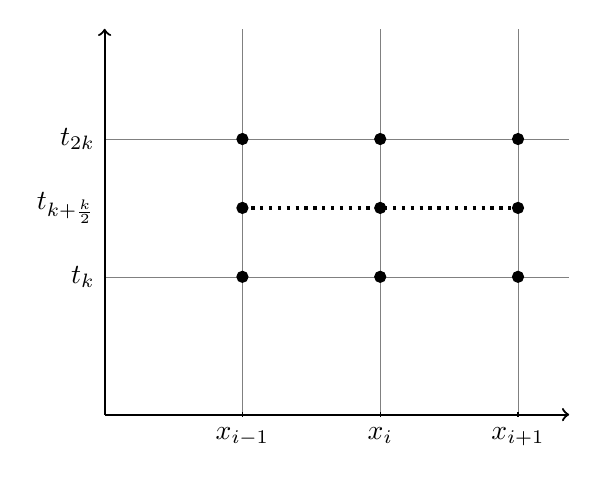
\begin{tikzpicture}
    \draw[step=1.75cm,gray,very thin] (0,0) grid (5.9,4.9);
    \draw[thick,->] (0,0) -- (5.9,0);
    \draw[thick,->] (0,0) -- (0,4.9);
    \draw[very thick, dotted] (1.75cm,2.625cm) -- (5.25cm,2.625cm);
    \draw (1.75cm, 1pt) -- (1.75cm, -1pt) node[anchor=north] {$x_{i-1}$};
    \draw (3.5cm, 1pt) -- (3.5cm, -1pt) node[anchor=north] {$x_{i}$};
    \draw (5.25cm, 1pt) -- (5.25cm, -1pt) node[anchor=north] {$x_{i+1}$};
 
    \draw (0pt, 1cm) -- (0pt, 1.75cm) node[anchor=east] {$t_{k}$};
    \draw (0pt, 2.5cm) -- (0pt, 2.625cm) node[anchor=east] {$t_{k+\frac{k}{2}}$};
    \draw (0pt, 3cm) -- (0pt, 3.5cm) node[anchor=east] {$t_{2k}$};
    
    \filldraw[black] (1.75cm,1.75cm) circle (2pt) node[anchor=west] {};
    \filldraw[black] (1.75cm,2.625cm) circle (2pt) node[anchor=west] {};
    \filldraw[black] (1.75cm,3.5cm) circle (2pt) node[anchor=west] {};
    \filldraw[black] (3.5cm,1.75cm) circle (2pt) node[anchor=west] {};
    \filldraw[black] (3.5cm,2.625cm) circle (2pt) node[anchor=west] {};
    \filldraw[black] (3.5cm,3.5cm) circle (2pt) node[anchor=west] {};
    \filldraw[black] (5.25cm,3.5cm) circle (2pt) node[anchor=west] {};
    \filldraw[black] (5.25cm,2.625cm) circle (2pt) node[anchor=west] {};
    \filldraw[black] (5.25cm,1.75cm) circle (2pt) node[anchor=west] {};
\end{tikzpicture}
\end{center}

We again use iteration of the implicit formula to obtain a result very close to the original vector, and again terminate the process once either of the two stopping conditions are met.
\newline
To derive the implicit formula for the half time-steps first we solve for components of the NLSE in terms of the half time-steps:
\begin{align*}
    [U_i^{n+1/2}]_t &\approx\frac{U_i^{n+1} - U_i^n}{h}\\
    [U_i^{n+1/2}]_{xx} &\approx \frac{U_{i-1}^{n+\frac{1}{2}} - 2 U_i^{n+\frac{1}{2}} +U_{i+1}^{n+1}}{h^2}\\
    [U_i^{n+1/2}]_{xx} &\approx \frac{U_{i-1}^{n} + U_{i-1}^{n+1} - 2(U_i^n + U_i^{n+1}) + (U_{i+1}^n + U_{i+1}^{n+1})}{2h^2}\\
    [U_i^{n+1/2}]_{xx} &\approx \frac{1}{2h^2}(A U^{n+1} + A U^n)\\
    U_i^{n+\frac{1}{2}}|U_i^{n+\frac{1}{2}}| &\approx \frac{1}{8}(U_i^n+U_i^{n+1})|U_i^n+U_i^{n+1}|
\end{align*}
By using these second scheme with these new time steps we obtain:
\[
    U^{n+1} - \frac{ik}{2h^2}AU^{n+1} = U^n + \frac{ik}{2h^2}AU^{n} +  \frac{ik}{4}(U_i^n+U_i^{n+1})|U_i^n+U_i^{n+1}|^2
\]
We can then simplify this equation by allowing:
\begin{align*}
    B_- &= I - \frac{ik}{2h^2}A\\
    B_+ &= I + \frac{ik}{2h^2}A\\
    F(U^n,U^{n+1}) &= \frac{ik}{4}(U_i^n+U_i^{n+1})|U_i^n+U_i^{n+1}|^2
\end{align*}
This results in the following simplification:
\begin{align*}
    B_- U^{n+1} &= B_+ U^n + F(U^n,U^{n+1})\\
    U^{n+1} &= B_-^{-1}(B_+ U^n + F(U^n,U^{n+1}))
\end{align*}
Then using iteration on both sides by letting $V_o = U^n$ and $V = U^{n+1}$ and solving the following in each iteration:
\[ V_{\ell+1} = B_-^{-1}(B_+ U^n + F(U^n,V_{\ell}))\]
We continue until one of our two conditions are met and assign the final value for $V_{\ell +1}$ to $U^{n+1}$.


\section{Experiment 1 - Sech(x)}
In the following subsections we test our numerical schemes for NLSE on the initial condition $U(x,0) = sech(x)$ which has been shown to be a very stable initial condition for the NLSE. This is because as time increases, the NLSE in theory will remain equal to the $sech(x)$ function.
\subsection{NLS1}
In this trial we use the initial condition that $U(x,0) = sech(x)$ and $x$ ranges from $-\frac{L}{2}$ to $\frac{L}{2}$ for $L= 20$ in increments of $h := L/N$ for $N = 2^7 = 128$. We evaluate in time step increments of $k = 1 \times 10^{-4}$.

\begin{figure}[H]
    \centering
    \includegraphics[width=\linewidth, height = 8cm]{nls1sechfinal.png}
    \caption{We can see that this scheme becomes inaccurate at $t = 15$.}
    \label{fig:my_label}
\end{figure}

It should be noted that for the following initial conditions, the average time this scheme took was 5.3106 seconds averaged over 30 runs. In the following experiments we will see that NLS1 is the worst of the three schemes. It is the most inaccurate, and as a consequence it requires smaller $k$ values to produce a scheme comparable to that of NLS2 or Crank-Nicholson. This smaller $k$ values translate to more work done by the CPU.

\subsection{NLS2}
In this trial we use all the initial conditions that we used in NLS1, but the only difference from the NLS1 experiment, is that instead of using time steps of $k = 1 \times 10^{-4}$ we will be using $k = \frac{1}{4}h^2$ which makes $k$ a function of $h$.
\begin{figure}[H]
    \centering
    \includegraphics[width=\linewidth, height = 8cm]{nlse2sechfinal.png}
    \caption{We can see that this scheme is much more accurate, and is able to last for more than 30 seconds. It should be noted however that the maximum values of $U$ suffer a slight decrease as the value of $t$ increases.}
    \label{fig:nls2sech}
\end{figure}

The decrease in the maximum values of $|U(x,t)|$ with increasing time mentioned in Figure \ref{fig:nls2sech}, can also be seen in the graphs of constants $M$ and $N$, in Figure \ref{nlsExp1M}, and Figure \ref{nlsExp1N} respectively. Despite the slight decrease in the maximum values for $|U(x,t)|$ with respect to increasing time, we conclude that NLS2 is a fairy good approximation of NLSE. It is also important to note that the average time that the script took (averaged over 200 runs) is 1.4907 seconds which is significantly shorter than how long NLS1 took.


\subsection{Crank-Nicholson}
We now examine the Crank-Nicholson scheme for approximating the NLSE. The average time that this scheme took over 200 trials is 1.84566, this shows that it takes slightly longer than the NLS2 scheme.
\begin{figure}[H]
    \centering
    \includegraphics[width=\linewidth, height = 8cm]{cnsechfinal.png}
    \caption{We see that this scheme is very accurate, and does not feature the steady decreasing that appeared in the NLS2 scheme.}
    \label{fig:my_label}
\end{figure}

\subsection{Conclusion of Experiment 1}
Below is the data for the Constants of Motion using the Sech(x) initial conditions.

\begin{figure}[H]
    \begin{subfigure}{0.5\textwidth}
    \centering\captionsetup{width=.85\linewidth}
        \includegraphics[width=0.8\linewidth, height=6cm]{images&graphs/MSech.png}
        \caption{Constant of Motion M}
        \label{nlsExp1M}
    \end{subfigure}%
    \begin{subfigure}{0.5\textwidth}
    \centering\captionsetup{width=.85\linewidth}
        \includegraphics[width=0.8\linewidth, height=6cm]{images&graphs/NSech.png}
        \caption{Constant of Motion: N}
        \label{nlsExp1N}
    \end{subfigure}
\caption{Constants of Motion for Sech(x) Initial Condition}
\label{fig:image2}
\end{figure}

\begin{figure}[H]
    \begin{subfigure}{0.5\textwidth}
    \centering\captionsetup{width=.85\linewidth}
        \includegraphics[width=0.8\linewidth, height=6cm]{images&graphs/errorMsech.png}
        \caption{Error of Constant: M}
        \label{NLS1 Mesh}
    \end{subfigure}
    \begin{subfigure}{0.5\textwidth}
    \centering\captionsetup{width=.85\linewidth}
        \includegraphics[width=0.8\linewidth, height=6cm]{images&graphs/errorNSech.png}
        \caption{Error of Constant: N}
        \label{NLS1 Constants of Motion}
    \end{subfigure}
\caption{Error of Constants of Motion for Sech(x) Initial Condition}
\label{fig:image2}
\end{figure}
For the log error of the constants we see that both the $M$ and $N$ constants stay roughly near their initial errors, and that for the Crank-Nicholson scheme the error of the $N$ constant is around $3$ orders of magnitude higher than the $M$ constant's. This is because of the error introduced from our central difference approximation of $U$'s $x-$derivative. Although all of our schemes use this central difference approximation, it can only be viewed with the Crank-Nicholson scheme because of how accurate this scheme is, the other schemes mask this error.

We conclude that the substantial differences in error makes up for the slightly longer CPU time required to run Crank-Nicholson in comparison to the NLS2 scheme, and so Crank-Nicholson should perform the best out of the three schemes in the experiments to come.
\vspace{1.25cm}

\section{Experiment 2 - One Bump}
In this experiment we test our schemes on the initial function:
\begin{equation*}
u(x, 0) &= a\big[1+rcos(\mu x)\big]
\end{equation*}
Where we let $a=0.5 , r = 0.01, \mu = 2pi/L, L = 2\sqrt{2} \pi$.
\vspace{1cm}

\subsection{NLS1}
Testing the first scheme under these conditions we found that we had to drastically increase the number of time steps between integer times from $k = 10^{-4}$ to $k = 4\times10^{-6}$ just to get a scheme that lasted for 15 seconds. We will see that this must also be done for the two bump initial condition as well. 

\begin{figure}[H]
    \centering
    \includegraphics[width=\linewidth, height = 8cm]{nls1onebumpfinal.png}
    \caption{We can see that the scheme becomes inaccurate at $t=15$.}
    \label{fig:exp2surf}
\end{figure}

It should be noted that due to the drastically increased number of time steps that the run-time of this scheme increased as well. From only taking 5.3106 seconds in experiment one, NLS1 with $k=4*10^{-6}$ takes a staggering 125.26 seconds. 

\subsection{NLS2}
For the NLS2 scheme we go back to using $k=\frac{1}{4}h^2$ for the the time step constant. For reference this comes out to be $k=.0012047$ roughly 300 times the size of the time constant for NLS1.
\vspace{1cm}
\begin{figure}[H]
    \centering
    \includegraphics[width=\linewidth, height = 8cm]{finalpicture.png}
    \caption{Here we can see that our second scheme is much more stable for the One Bump initial condition. NLS2 succeeds in lasting the full 30 seconds.}
    \label{fig:exp2nls2}
\end{figure}

This scheme allows us a better time constant, and as a result only takes 5.195 seconds averaged for a 100 trials. So not only is the scheme accurate for twice as long (independent trials showed that it could last for 500 seconds without ever incurring error greater than order $5\times10^{-1}$), but the run-time needed for the scheme is nearly 20 times less than that needed for NLS1.

While this scheme does reach a large error it returns to an extremely low error at approximately $t = 10$ seconds. As the scheme continues it again creates a large error before again becoming a good approximation at around $t = 30$ seconds. \\

\subsection{Crank-Nicholson}
When we apply the Crank-Nicholson scheme to the same boundary conditions we obtain the following surface:

\begin{figure}[H]
    \centering
    \includegraphics[width=\linewidth, height = 8cm]{cnonebumpfinal.png}
    \caption{Notice that this surface only has one peak vs. the two peaks that appear in NLS2. It should be noted that the max value at the peak is approximately 1.2}
    \label{fig:exp2surf}
\end{figure}

We find this to be the most accurate scheme. It features only slightly longer run-time requirements than NLS2 (6.5 seconds averaged over 100 runs), but offers a much more accurate surface. 
\vspace{1.5cm}
\subsection{Conclusion - One Bump}

Below is the data for the Constants of Motion and their errors for the one bump initial condition. The error plots for the constants of motion confirm that the Crank-Nicholson scheme is the best of our three schemes.

\begin{figure}[H]
    \begin{subfigure}{0.5\textwidth}
        \centering\captionsetup{width=.85\linewidth}%
        \includegraphics[width=0.8\linewidth, height=6cm]{images&graphs/onebumpM.png}
        \caption{Constant of Motion: M}
        \label{NLS1 Mesh}
    \end{subfigure}
    \begin{subfigure}{0.5\textwidth}
        \centering\captionsetup{width=.85\linewidth}%
        \includegraphics[width=0.8\linewidth, height=6cm]{images&graphs/onebumpN.png}
        \caption{Constant of Motion: N}
        \label{NLS1 Constants of Motion}
    \end{subfigure}
\caption{Constants of Motion for the One Bump initial condition}
\label{fig:image2}
\end{figure}

\begin{figure}[H]
    \begin{subfigure}{0.5\textwidth}
        \centering\captionsetup{width=.85\linewidth}%
        \includegraphics[width=0.8\linewidth, height=6cm]{images&graphs/errMonebump.png}
        \caption{Log Error of M}
        \label{NLS1 Mesh}
    \end{subfigure}
    \begin{subfigure}{0.5\textwidth}
        \centering\captionsetup{width=.85\linewidth}%
        \includegraphics[width=0.8\linewidth, height=6cm]{images&graphs/errNonebump.png}
        \caption{Log Error of N}
        \label{NLS1 Constants of Motion}
    \end{subfigure}
\caption{Log Error of Constants for the One Bump initial condition.}
\label{fig:image2}
\end{figure}
We noticed that although both NLS2 and Crank-Nicholson are accurate for much longer than NLS1, that NLS2 produced a very different surface than Crank-Nicholson's. This is because that although NLS2 has small error (order $10^{-2})$, it is still nearly 100 times that of Crank-Nicholson's at the later time periods. We might be led to believe that an error of order $10^{-2}$ is pretty good, but this experiment proves otherwise since this error produces a drastically different surface.
\newline
Another interesting thing that we see from the error plots is that the error increases at times, but then shrinks at later times. Our hypothesis is that this is caused from the surface peaks. We believe that the errors are masked by the function $|U(x,t)|$ decreasing after its peak. Since the NLS2 surface has an additional peaking time for $|U(x,t)|$ than the Crank-Nicholson scheme, that the NLS2 error does not benefit from this mask. 

\section{Experiment 3 - Competing Waves}
For this experiment we test our schemes with the initial function of competing waves. This equation is:
\begin{equation*}
    U(x,0) = \frac{1}{2}\Bigg[1 + r_1cos\bigg(\frac{2\pi}{L}x\bigg) + r_2cos\bigg(\frac{4pi}{L}\Big(x-\frac{L}{4}\Big)\bigg)\Bigg];
\end{equation*}
where $L = 4\pi\sqrt{2}$, $N = 128$, $h = \frac{L}{N}$, and $k = \frac{1}{4}h^2$. For the following trials we keep the constant $r_1 = .1$ fixed while we examine changing values for $r_2$. The values of $r_2$ come from the set $S = \{.009,.025,.0375,.1\}$.

\subsection{Competing Waves with Crank-Nicholson}
\begin{figure}[H]
    \begin{subfigure}{0.5\textwidth}
        \centering\captionsetup{width=.85\linewidth}%
        \includegraphics[width=0.8\linewidth, height=6cm]{009.png}
        \caption{Here we have set $r_2 = .009$. We examine the graph of $U(x,t)$ from the side and see that the \textit{strong} wave is in front of the weak wave. }
        \label{NLS1 Constants of Motion}
    \end{subfigure}
    \begin{subfigure}{0.5\textwidth}
        \centering\captionsetup{width=.85\linewidth}%
        \includegraphics[width=0.8\linewidth, height=6cm]{025.png}
        \caption{We now set $r_2 = .025$, and see that the \textit{strong} wave is now closer to the \textit{weak} wave.}
        \label{NLS1 Constants of Motion}
    \end{subfigure}
\caption{Competing Waves.}
\label{fig:image2}
\end{figure}

\begin{figure}[H]
    \begin{subfigure}{0.5\textwidth}
        \centering\captionsetup{width=.85\linewidth}%
        \includegraphics[width=0.8\linewidth, height=6cm]{0375.png}
        \caption{Now we set $r_2 = .0375$ and see that the two waves have now coalesced and have gone through constructive interference.}
        \label{NLS1 Mesh}
    \end{subfigure}
    \begin{subfigure}{0.5\textwidth}
        \centering\captionsetup{width=.85\linewidth}%
        \includegraphics[width=0.8\linewidth, height=6cm]{1.png}
        \caption{Finally we set $r_2 = .1$, and see that the \textit{strong} wave has swapped positions with the \textit{weak} wave.} 
        \label{NLS1 Constants of Motion}
    \end{subfigure}
\label{fig:image2}
\caption{Competing Waves(continued).}
\end{figure}

These four graphs exhibit the \textit{rogue} wave phenomenon, where the nonlinear term in the Schr\"odinger Equation takes effect, and the \textit{strong} wave takes in energy from the \textit{weak} wave using this to bolster its own peak.


\subsection{Competing Waves with NLS2}
For this experiment we test NLS2 only with the $r_2 = .0375$. This is because $r_2 = .0375$ is the critical $r_2$ value that demonstrates the \textit{rogue wave} phenomenon, and that Crank-Nicholson has proven to be a better approximation of NLSE.

\begin{figure}[H]
    \begin{subfigure}{0.5\textwidth}
        \centering\captionsetup{width=.85\linewidth}%
        \includegraphics[width=0.8\linewidth, height=6cm]{images&graphs/nlse2twobump.png}
        \caption{Mesh of NLS2 with $r_2 = .0375$}
        \label{EXP3 NLS2 Side}
    \end{subfigure}
    \begin{subfigure}{0.5\textwidth}
        \centering\captionsetup{width=.85\linewidth}%
        \includegraphics[width=0.8\linewidth, height=6cm]{images&graphs/exp3nls2side.png}
        \caption{Side view of (a). We see that NLS2 with the Two Bump initial condition follows the trend of decreasing with time.}
        \label{EXP3 NLS2 Error}
    \end{subfigure}
\label{fig:image2}
\caption{NLS2 Mesh Side-View \& Log Error}
\end{figure}

\subsection{Competing Waves with NLS1}
In this section we attempt to use the competing waves initial condition with the NLS1 scheme. We see that even by decreasing the size of the time steps and increments in the x value, that we still cannot get an accurate approximation with this scheme. $k = 5\times 10^{-5}$, we get the following surface for $r_2 = 0.0375$:

\begin{figure}[H]
    \centering
    \includegraphics[width=\linewidth, height = 8cm]{images&graphs/nls1twobump.png}
    \label{fig:exp2surf}
\end{figure}

Interestingly, the NLS1 scheme works better with the two bump initial condition than it does with the one bump initial condition. Although it only lasts for 15 seconds, it accomplishes this with an improved time constant. This improved time constant translates to an average time per trial of 9.2 seconds (averaged over 100 trials) compared to 125 seconds for the one bump initial condition.
\subsection{Conclusion - Two Bump}
The Constants of Motion and their errors for the two bump initial condition are displayed below:
\begin{figure}[H]
    \begin{subfigure}{0.5\textwidth}
        \centering\captionsetup{width=.85\linewidth}%
        \includegraphics[width=0.8\linewidth, height=6cm]{images&graphs/twobumpM.png}
        \caption{Constant of Motion: M}
        \label{EXP3 NLS2 Side}
    \end{subfigure}
    \begin{subfigure}{0.5\textwidth}
        \centering\captionsetup{width=.85\linewidth}%
        \includegraphics[width=0.8\linewidth, height=6cm]{images&graphs/twobumpN.png}
        \caption{Constant of Motion: N}
        \label{EXP3 NLS2 Error}
    \end{subfigure}
\label{fig:image2}
\caption{Constants of Motion for Two Bump initial condition.}
\end{figure}
\begin{figure}[H]
    \begin{subfigure}{0.5\textwidth}
        \centering\captionsetup{width=.85\linewidth}%
        \includegraphics[width=0.8\linewidth, height=6cm]{images&graphs/twobumperrM.png}
        \caption{Log Error of M}
        \label{EXP3 NLS2 Side}
    \end{subfigure}
    \begin{subfigure}{0.5\textwidth}
        \centering\captionsetup{width=.85\linewidth}%
        \includegraphics[width=0.8\linewidth, height=6cm]{images&graphs/twobumperrN.png}
        \caption{Log Error of N}
        \label{EXP3 NLS2 Error}
    \end{subfigure}
\label{fig:image2}
\caption{Log Error of Constants of Motion}
\end{figure}

From these plots we see that again Crank-Nicholson is the best of the three schemes, and that the NLS2 scheme continues with this trend of shrinking over time. Furthermore we found that the NLS1 scheme performed surprisingly better than it had with the one bump initial condition. Finally we have seen that the \textit{rogue wave} phenomenon appears in all three of these schemes, even if only for a moment (NLS1 blew up directly after). 

\section{Experiment 4 per1}
For this experiment we test our schemes with the initial function of per1 that comes from . This equation is:
\begin{equation*}
    U(x,t) = \dfrac{ae^{2a^2it)}(1 - 4( 1 + 4it)}{ 1 + 16t^2 + 4x^2}
\end{equation*}
where $L = 4\pi\sqrt{2}$, $N = 128$, $h = \frac{L}{N}$, and $k = \frac{1}{4}h^2$. 

\section{Conclusion}
From the application of these three schemes to varying initial conditions we can see just how important choosing a scheme can be. We found that the Crank-Nicholson scheme is the most accurate of our three schemes, while only coming at a marginal cost in terms of actual run-time. While there is still a certain degree of error in all of these schemes, the schemes themselves vary greatly in performance and CPU time. Further study into derivation and testing of new schemes may yield better approximations in the future that can be more generally applied.
\end{document}